\documentclass[xcolor=dvipsnames,aspectratio=169]{beamer}

% INCLUSIÓN DOS PAQUETES IMPRESCINDIBLES DE IDIOMA E CODIFICACIÓN DE CARACTERE.
\usepackage[T1]{fontenc}
\usepackage[english]{babel}
\usepackage[utf8]{inputenc}
\usepackage{csquotes}

%ACRONYMS para engadir un glosario de acronimos automatizado
% \usepackage[acronyms,nonumberlist,nopostdot,nomain,nogroupskip]{glossaries}
% \input{./acronyms.tex}

% PAQUETES PARA FIGURAS E GRAFICOS
\usepackage{graphicx}
%   \usepackage[pdftex]{graphicx}
  \usepackage{epstopdf}
   \graphicspath{{./img/}}
  % and their extensions so you won't have to specify these with
  % every instance of \includegraphics
   \DeclareGraphicsExtensions{.eps,.pdf,.png,.jpg}   
\usepackage{subfigure}
\usepackage{caption}

%Tikz plots
\usepackage{tikz}
\usepackage{tikzscale}
\usetikzlibrary{plotmarks,patterns,decorations.pathreplacing,backgrounds,calc,arrows,arrows.meta,spy,matrix,backgrounds}
\newcommand{\tikzmark}[1]{\tikz[overlay,remember picture] \UE (#1) {};}
\newcommand{\DrawBox}[4][]{%
    \tikz[overlay,remember picture]{%
        \coordinate (TopLeft)     at ($(#2)+(-0.4em,1.6em)$);
        \coordinate (BottomRight) at ($(#3)+(0.4em,-1.0em)$);
        %
        \path (TopLeft); \pgfgetlastxy{\XCoord}{\IgnoreCoord};
        \path (BottomRight); \pgfgetlastxy{\IgnoreCoord}{\YCoord};
        \coordinate (LabelPoint) at ($(\XCoord,\YCoord)!0.5!(BottomRight)$);
        %
        \draw [red,#1] (TopLeft) rectangle (BottomRight);
        \UE [below, #1, fill=none, fill opacity=1] at (LabelPoint) {#4};
    }
}
\usepackage{pgfplots}
\pgfplotsset{compat=newest}
\pgfplotsset{plot coordinates/math parser=false}
\usepgfplotslibrary{patchplots,groupplots}

% OUTROS PAQUETES DE USO COMUN. HOXE EN DIA OS COMPILADORES SON TAN RAPIDOS QUE EU METO TODOS SEMPRE
% \usepackage{float}
% \usepackage{ucs} 
% \usepackage{subcaption}
\usepackage{psfrag}
\usepackage{verbatim}
\usepackage{amsmath}
\usepackage{amsfonts} 
\usepackage{amssymb} 
\usepackage{amsthm}
\usepackage{pifont}
\usepackage{array}
\usepackage{listings}
\usepackage{stfloats}
\usepackage{algorithm} 
\usepackage{algorithmic} 
\usepackage{url} 
\usepackage{enumerate}
\usepackage{multirow}
\usepackage{wasysym}
\usepackage{cancel}
\usepackage{lmodern}

\input{EETbeamerconfig.tex}
\input{mydefinitions.tex}

%---------------
% LIMIAR
%---------------
%configuracion de opcions de beamer persoais, pero alleas ao estilo

% COMANDO QUE INTRODUCE UNHA DIAPOSITIVA CUN ÍNDICE NO QUE APARECEN VELADAS TÓDALAS SECCIÓNS MENOS A ACTUAL. ÚTIL PARA INTRODUCIR OS TÍPICOS ÍNDICES INTERMEDIOS.
\newcommand{\Inter}{\frame{\tableofcontents[currentsection]}}
\newcommand{\inter}{\frame{\tableofcontents[currentsection,currentsubsection]}}

% Pes de imaxe
\renewcommand{\figurename}{Fig.}
\addto\captionsenglish{\renewcommand{\figurename}{Fig.}}
\setbeamertemplate{caption}[numbered]

%ESTE PAQUETE PERMITE POÑER A BIBLIOGRAFIA AO PE DE PAXINA CON CONFIGURACIONS ESTETICAS PERSOAIS
% \usepackage[style=ieee,doi=false,isbn=false,url=true,backend=bibtex]{biblatex}
% \bibliography{./bibliografia.bib}
% \newrobustcmd*{\footfullcitenomark}{%
%   \AtNextCite{%
%     \let\thefootnote\relax 
%     \let\mkbibfootnote\mkbibfootnotetext
%     }%
%   \footfullcite}

%paquete para engadir notas de guion ao pdf
\usepackage{pgfpages}
% \setbeameroption{show only notes} 
% \setbeameroption{show notes}
% \setbeameroption{show notes on second screen=right}
% DATOS DO DOCUMENTO
\title{Advanced Communication Systems}
\subtitle{Part 2.0:\\ Multi-user Communications:\\ Information Theory Recap}
\author[FGC]{Felipe G\'omez Cuba}
\institute[XX]{
\begin{columns}[T]
\begin{column}{9cm}\centering
Despacho 204\\
Titorías: Lun-Xov 15:00-16:30\\
(En caso de confinamento: videochamada a calquera horario acordado)\\
  \texttt{gomezcuba@gts.uvigo.es}\\
\end{column}
\end{columns}
}

\date{22 October 2020 }
\begin{document}

% Diapositiva co título
%\frame[plain]{\titlepage}%the ``classic'' beamer cover pageç

\frame{\frametitle{\\}%generate top bar, but blank line as tittle
\titlepage
}%approximation to the ``GPSC ppt'' cover page, but with central beamer title

% \frame{\tableofcontents}
% \note[itemize]{%itemized notes are special ``note'' slides that beamer can append to the pdf or not, depending on a boolean toggle option
% \item Introduce yourself
% \item In this work we studied blablabla.
% }

% \section{IAB MmWave Network}

\frame{\frametitle{Entropy}
    \begin{definition}
    The \textbf{entropy} of a random variable $X$ with a probability mass function $p(x)$ defined over a \textit{discrete} support set $x\in\mathcal{X}$ is given by
    \begin{equation}
     \Ent{X}=-\Ex{X}{\log(p(x))}=-\sum_{x\in\mathcal{X}}p(x)\log(p(x))
    \end{equation}
    \end{definition}
    \begin{itemize}
     \item $\Ent{X}\geq 0$
     \item $\Ent{X}\leq \log(|\mathcal{X}|)$
    \end{itemize}
}
\frame[allowframebreaks]{\frametitle{Entropy Examples}
    \begin{itemize}
     \item Let $X=\begin{cases}a&\textnormal{w.p. }p\\b&\textnormal{w.p. }1-p\end{cases}$ then $$\Ent{X}=-p\log(p)-(1-p)\log(1-p)\leq 1 (bits)$$
     \begin{figure}[!h]
      \includegraphics[width=.5\columnwidth]{coverHp}
      \caption{credit: Thomas \& Cover}
      \end{figure}
     \item Let $X=\begin{cases}a&\textnormal{w.p. }\frac{1}{2}\\b&\textnormal{w.p. }\frac{1}{4}\\c&\textnormal{w.p. }\frac{1}{8}\\d&\textnormal{w.p. }\frac{1}{8}\\ \end{cases}$ then
                   $$\Ent{X}=\frac{7}{4} (bits)$$
      \textbf{Optimal Source Coding (Huffman)}: Let a code be $a\to 0$, $b\to 10$, $c\to 110$, $d\to 111$, then the avg. message length is
      $$1\frac{1}{2}+2\frac{1}{4}+3\frac{1}{8}+3\frac{1}{8}=\frac{7}{4} (bits)$$
                   
    \end{itemize}
}
\frame{\frametitle{Diferential Entropy}
    \begin{definition}
    The \textbf{diferential entropy} of a r.v. $X$ with a probability density function $f(x)$ defined over a \textit{continuous} support set $x\in\mathcal{X}$ is
    \begin{equation}
     h(X)=-\Ex{X}{\log(p(x))}=-\int_{x\in\mathcal{X}}p(x)\log(p(x))
    \end{equation}
    \end{definition}
    \begin{itemize}
     \item \textcolor{ARust}{$\cancel{h(X)\geq 0}$}
     \item Careful with $+C$ in the integral!
    \end{itemize}
    \begin{theorem}
     Among all random variables with support in $\mathcal{X}=\mathbb{R}$, zero mean and variance $\sigma^2$, the entropy is maximized if $X$ is Gaussian
     \begin{equation}
      \begin{split}
       \max_{f(x)}&\; h(x)\\ \;\textnormal{s.t. }&\Ex{X}{x}=0\textnormal{ and } \Ex{X}{x^2}=\sigma^2
      \end{split} \Leftrightarrow \mathcal{N}(0,\sigma^2)
     \end{equation}
    \end{theorem}
}
\frame[allowframebreaks]{\frametitle{Entropy of Multiple Variables}
    \begin{definition}
    The \textbf{joint entropy} of a pair of r.v. $(X,Y)$ is
     $$\Ent{X,Y}=-\sum_{(x,y)\in\mathcal{X}\times\mathcal{Y}}p(x,y)\log(p(x,y))$$
    \end{definition}
    \begin{itemize}
     \item Complex numbers $z \triangleq (\Re\{z\},\Im\{z\})$
     \item Vectors $\x\in \mathbb{C}^N \triangleq (x_1,x_2,\dots x_N)$
    \end{itemize}
    \begin{theorem}
     Among and random variables $X$ with support in $\mathbb{C}^N$, zero mean and covariance matrix $\Sb$, the entropy is maximized if $X$ is $\mathcal{CN}(0,\Sb)$
     \end{theorem}
     \begin{remark}[p.d.f. of $\mathcal{CN}(\vec{\mu},\Sb)$]
        $f(\x)=\pi^{-N}\det(\Sb)^{-1}e^{-(\x-\vec\mu)^H\Sb^{-1}(\x-\vec\mu)}$
     \end{remark}


     \pagebreak
    \begin{definition}
    The \textbf{conditional entropy} of r.v. $X$ conditioned on $Y$ is    
     $$\CEnt{X}{Y}=\Ex{p(y)}{\Ent{X|Y=y}}=-\sum_{(x,y)\in\mathcal{X}\times\mathcal{Y}}\textcolor{ARust}{p(x,y)}\log(p(x|Y=y))$$
    \end{definition}
    \begin{theorem}[Chain Rule]
        $$\Ent{X,Y}=\Ent{X}+\CEnt{Y}{X}$$
    \end{theorem}
    \begin{theorem}[Conditioning Reduces Entropy]
        $$\Ent{X}\geq\CEnt{X}{Y}$$
    \end{theorem}
}
\frame[allowframebreaks]{\frametitle{Measuring Information}
    \begin{definition}
        The \textbf{mutual information} between two r.v. $X$ and $Y$ is
        $$\Inf{X}{Y}=\Ent{X}-\CEnt{X}{Y}=\int_x\int_yf(x,y)\log\left(\frac{f(x,y)}{f(x)f(y)}\right)$$
    \end{definition}
    ``How much uncertainty of $X$ decreases if we know $Y$''
    
    \begin{theorem}[Channel Capacity]
        For dependent r.v. $Y$ as a function of r.v. $X$ the maximum rate of \textbf{reliable} communication through the channel $f(Y|X)$ is
        $$C=\sup_{f(x)} \Inf{X}{Y}\textnormal{  s.t.  (constraints)}$$
    \end{theorem}
    
    \begin{itemize}
     \item Binary Simmetric Channel (BSC):
     $$Y=\begin{cases}
                                               X&\textnormal{w.p. } 1-p\\
                                               \textnormal{not}(X)&\textnormal{w.p. } p
                                              \end{cases}$$
     with constraint $X\in\{0,1\}$
     $$C_{BSC}=1-H(p)$$\\ \ \\
     \item Additive White Gaussian Noise (AWGN) real channel:
     $$y=x+z,$$
     with $z\sim\mathcal{N}(0,\sigma^2)$, $\x\in\mathbb{R}$, and $\Ex{}{|X|^2}=P$
     $$C_{AWGN}=\frac{1}{2}\log(1+\frac{P}{\sigma^2})$$\\ \ \\

    \end{itemize}
}

\frame[allowframebreaks]{\frametitle{Complex AWGN MIMO DEC}
\begin{figure}
 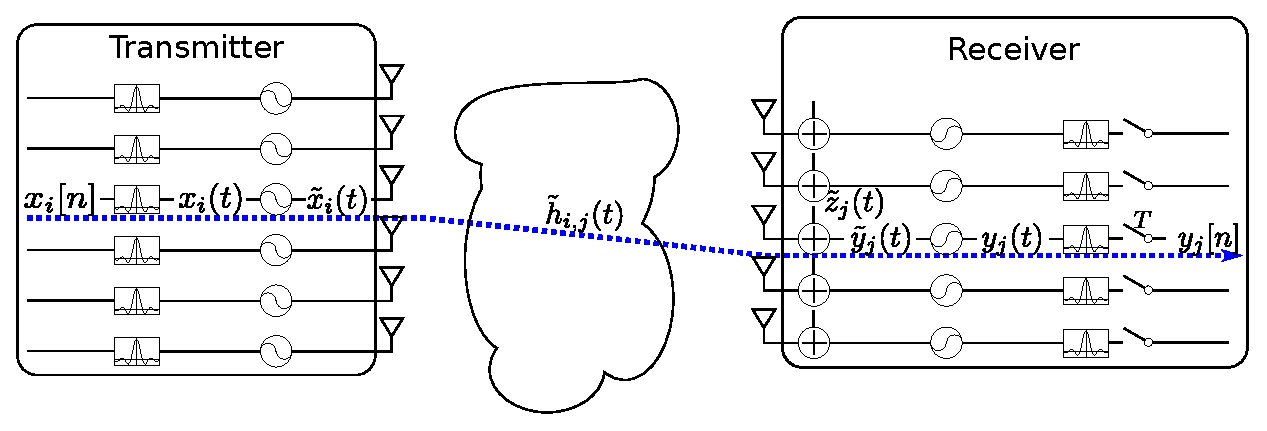
\includegraphics[width=.75\columnwidth]{channel}
\end{figure}

\begin{itemize}
 \item Assume a transmitter with $N_t$ transmit antennas.
 \item The RF real signal sent by the $i$-th antenna is 
 $$\tilde{x}_i(t)=\Re\{x_i(t)e^{-jf_ct}\}$$
 \pagebreak
 \item Assume a receiver with $N_r$ receive antennas.
 \item The RF real channel from the $i$-th tx. to the $j$-th rx antenna is 
 $$\tilde{y}_j(t)=\tilde{h}_{j,i}(t)*\tilde{x}_i(t)+\tilde{z}(t)$$
 \item Example: multipath channel
     $$\tilde{h}_{j,i}(t)=0.8\delta(t)+0.6e^{j\pi/3}\delta(t-2\mu s)$$     
     \pagebreak
 \item Digital discrete-time transmission: $$x_i(t)=\sum_{n=-\infty}^{\infty}x_i[n]p(t-nT)$$
 \item Frequency change and receive filter: $$y_j(t)=g(t)*\left(\tilde{y}_j(t)e^{jf_ct}\right)$$
 \item Sampling receiver: $$y_j[n]=y_j(nT)$$
 \pagebreak
 \item Discrete Equivalent Channel:
    $$y_j[n]=\sum_{m}h_{i,j}[n-m]x_i[m]+z[n]$$
 \item If $g(t)$ meets Nyquist no-ISI criteron, $z[n]$ is AWGN
 \item If all multipath delays of $\tilde{h}_{j,i}(t)$ $\ll$ $T$, no ISI 
        $$y_j[n]\simeq h_{i,j}x_i[n]+z[n]$$
 \item Puting all pairs of antennas together (omitted $[n]$)
 $$\left(\begin{array}{c}y_1\\\vdots\\y_{N_r}\end{array}\right)=\left(\begin{array}{ccc}h_{1,1}&\dots&h_{1,N_t}\\\vdots&\ddots&\vdots\\h_{N_r,1}&\dots&h_{N_r,N_t}\end{array}\right)\left(\begin{array}{c}x_1\\\vdots\\x_{N_t}\end{array}\right)+\left(\begin{array}{c}z_1\\\vdots\\z_{N_r}\end{array}\right)$$
 \pagebreak
 \item \textbf{Multiple Input Multiple Output AWGN DEC}
    $$\y=\Hb\x+\z$$
 \item Capacity of the MIMO AWGN channel
    $$\sup_{f(\x)}\Inf{\x}{\y}$$
    \begin{itemize}
        \item With a fixed covariance matrix constraint $\Ex{}{\x\x^H}=\Sb_x$
            $$C(\Sb_x)=\log\det\left(\I+\frac{1}{\sigma_z^2}\Hb\Sb_x\Hb^H\right)$$
            \pagebreak
        \item Optimized covariance at tx. with no knowledge of $\Hb$
            \begin{equation}
            \label{eq:Ccsir}
                C=\sup_{\Sb_x}\{C(\Sb_x)\}=\log\det\left(\I+\frac{P}{N_t\sigma_z^2}\Hb\Hb^H\right)
            \end{equation}

            where optimum $\Sb_x$ is $\frac{P}{N_t}\I$.\\
            \textbf{CSIR: Channel State Information at the Receiver}\\ \ \\
        \item Optimized covariance at tx. with knowledge of $\Hb$
            \begin{equation}
            \label{eq:Ccsit}
                C=\sup_{\Sb_x|\Hb}\{C(\Sb_x)\}=\sum\log\left(1+\frac{P_i\lambda_i}{\sigma_z^2}\right)
            \end{equation}
            for $\lambda_i\in\textnormal{Eigen}(\Hb\Hb^H)$, $P_i=(\frac{1}{\beta}-\frac{\sigma_z^2}{\lambda_i})^+$, $\beta$ Lagrange multiplier.\\
            \textbf{CSIT: Channel State Information at the Transmitter}
    \end{itemize}
\end{itemize}
}

\frame[allowframebreaks]{\frametitle{Insights from Channel Capacity}

\begin{itemize}
    \item In Shannon's theorem Capacity $\triangleq\sup R$ \textbf{with probability of error as low as desired}.
    \begin{itemize}
    \item Let $\hat{x}=\textnormal{decode}(\y)$
    \item Channel is used $L_w$ times, $\{X[n]\}_{n=0}^{L_w}$ and $\{Y[n]\}_{n=0}^{L_w}$
    \item if $R>C$ then $\displaystyle \lim_{L_w\to\infty} P(\hat{x}\neq x) > 0 $
    \item if $R\leq C$ then $\displaystyle \lim_{L_w\to\infty} P(\hat{x}\neq x) = 0 $\\ \ \\
    \end{itemize}
    \item Gaussian Random Variable $f(\x)$: the Maximum-Likelihood (ML) detector is Least Squares
    $$\hat{\x} = \arg\max_{\x\in\mathcal{X}} f(\y|\x) = \arg\min_{\x\in\mathbb{C}^{N_t}} \|\y-\Hb\x\|^2$$
    \item Gaussian Codebook (random constellation) $f(\x)$: ML is NP-hard
    $$\hat{\x} = \arg\max_{\x\in\mathcal{X}} f(\y|\x) = \arg\min_{\x\in\textcolor{ARust}{\mathcal{C}^{N_t}}} \|\y-\Hb\x\|^2$$

 \item Discrete-time channel capacity is in units of bits/period $T$
 \item With sinc pulses $p(t)$ and $g(t)$, bandwidth is $B=1/T$
    $$C=\sup_{\Sb_x} B\log\det\left(\I+\frac{1}{N_oB}\Hb\Sb_x\Hb^H\right)(bps)$$
    with noise Power Spectral Density (PSD) $N_o$. \\ \ \\
 \item Spectral efficiency $\frac{C}{B}$ bits/s/Hz. \\ \ \\
 \item \textbf{Degrees of Freedom (DoF):}
 $$\lim_{\frac{P}{N_o}\to\infty} \frac{C}{\log(1+\frac{P}{N_o})} = B\rank(\Hb)\leq B\min(N_t,N_r)$$
 \pagebreak
 \item With small $B$ rate is limited by DoF 
 \item With large $B$ rate is limited by power 
 $$\lim_{B\to\infty} C(B)=\frac{P}{N_o}\log e$$
 \begin{figure}
\includegraphics[width=.35\columnwidth]{widebandcap} 
\end{figure}

 \item Minimum energy per transmitted bit $\frac{P/N_o}{C}\geq -\log_2 e = -1.56dB$. \\ \ \\
\end{itemize}
}

\frame{\frametitle{Capacity vs Real Decoder}
    \begin{itemize}
     \item We cannot generate a Gaussian $f(\x)$ in a real circuit\\ \ \\
     \item Define a ``M-QAM constrained Capacity''
        $$C_{M-QAM} = \sup_{f(\x)\textnormal{ s.t. }x_i\in\mathcal{C}_{M-QAM}} \Inf{\x}{\y}$$
     \item For some values of $P/N_o$ and $M$, $\mathcal{C}_{M-QAM}$ is similar to $C$
        \begin{figure}
        \includegraphics[width=.35\columnwidth]{capacityDiCo}
        \end{figure}
     \item Practical implementation:
     \begin{itemize}
        \item Carefully adjusted $M$ vs $P/N_o$ 
        \item Design algorithm $\hat{\x}=\textnormal{decode}(\y)$ with low $P(\hat{\x}\neq \x)$
    \end{itemize}
    \end{itemize}
}


\frame[allowframebreaks]{\frametitle{MIMO Receivers: Sphere Decoder}
    \begin{definition}
     Given a family of random variables $Y$ that depend on a parameter $\x$, the \textit{Likelihood Function} is the function that evaluates the p.d.f. of $Y$ with an observation $\y$ for different values of $\x$.
     $$\mathcal{L}_{\y}(\x)=f(Y=\y|\x)$$
    \end{definition}

    \begin{theorem}
     If symbols are equiprobable, the Maximum Likelihood detector achieves the minimum error probability.
     $$\min P(\hat{\x}\neq \x) \Leftrightarrow \hat{\x}=\arg\max_{\x\in\mathcal{C}^{N_t}} f(\y|\x)$$
    \end{theorem}
\pagebreak
    \begin{itemize}
     \item Consider a digital constellation $\mathcal{C}$ (BPSK, QAM, ...)
     \item $N_t$-dimension transmitted vector $\x\in\mathcal{C}^{N_t}$
     \begin{itemize}
        \item For $N_t=1$ the ML detector is the \textit{decisor} we are familiar with
        \item For $N_t>1$, the ML detector is a combinatorial problem\\ \ \\
     \end{itemize}
     \pagebreak
     \item Sphere Decoder (fast ML):
        \begin{itemize}
            \item Unconstrained ML decision $\overline{\x}=(\Hb^H\Hb)^{-1}\Hb^H\y$
             $$\arg\min_{\x\in\mathcal{C}^{N_t}} \|\y-\Hb\x\|^2 = \arg\min_{\x\in\mathcal{C}^{N_t}} (\overline{\x}-\hat{\x})^H\Hb^H\Hb(\overline{\x}-\hat{\x})$$
            \item Test only values of $\hat\x$ close to $\overline{\x}$, within radius $|\overline{\x}-\hat{\x}|^2\leq r$
            
                \begin{figure}
                \includegraphics[width=.45\columnwidth]{sphere}
                \caption{Credit: Luis Castedo Ribas}
                \end{figure}
        \end{itemize}
    \end{itemize}
}


\frame[allowframebreaks]{\frametitle{MIMO Receivers: Linear Receivers}
    \begin{itemize}
     \item General Structure:
     \begin{itemize}
        \item Multiply $\y$ by a linear matrix filter $\rr=\W\y$
        \item Design $\W$ mapping each $r_i$ to one transmitted symbol $x_i$
        \item Symbol-by-symbol decision $\hat{x}_i=\textnormal{map}(r_i,\mathcal{C})$\\ \ \\
     \end{itemize}
     \item Matched Filter: $\W=\Hb^H$\\ \ \\
     \item Zero Forcing channel equalizer: $\W=(\Hb^H\Hb)^{-1}\Hb^H$\\ \ \\
     \item Minimum Mean Squared Error eq.: $\W=(\Hb^H\Hb+\sigma_z^2\I)^{-1}\Hb^H$
    \end{itemize}
}

\frame[allowframebreaks]{\frametitle{MIMO Receivers: Non-Linear Receivers}
    \begin{itemize}
     \item QR decomposition of $\Hb=\Q\R$
     \begin{itemize}
        \item Orthogonal $\Q^H\Q=\I$
        \item Lower triangular $\R$\\ \ \\
    \end{itemize}
     \item Convert the channel to triangular 
        $$\rr=\Q^H\y=\R\x+\Q\z=\R\x+\z'$$
     \item Decision-Feedback
     \begin{itemize}
        \item $\hat{x}_1=\textnormal{map}(r_1,\mathcal{C})$
        \item Substract $R_{1,2}\hat{x}_1$ from $r_2$ and decide $x_2$
        \item iterate $\hat{x}_i=\textnormal{map}(r_i-\textnormal{cancel}(x_1\dots x_{i-1}),\mathcal{C})$
         $$\vv=\rr-(\R-\I)\hat{\x}\textnormal{ and }\hat{x}_i=\textnormal{map}(v_i,\mathcal{C})$$
     \end{itemize}
     \pagebreak
     \item Choleski decomposition $\Hb^H\Hb=\Lb^H\LL\Lb$
        \begin{itemize}
         \item $\Lb$ triangular with ones in diagonal
         \item $\LL$ diagonal matrix
         \item $\R=\LL^{\frac{1}{2}}\Lb$\\ \ \\
        \end{itemize}
     \item DF with Reordering:     
     \begin{itemize}
        \item Permute order of rows of $\Hb$
        \item Move up ``better'' channel gains (reorder $\LL$)
        \item Reduce error propagation
        \item Combinatorial!\\ \ \\
    \end{itemize}
     \item DF with MMSE: Choleski dec. $(\Hb^H\Hb+\sigma_z^2\I)=\Lb^H\LL\Lb$\\ \ \\
    \end{itemize}
}


\frame[allowframebreaks]{\frametitle{Fading}
    \begin{itemize}
     \item $h_{i,j}$ is a channel coefficient that stems from $\tilde{h}_{i,j}(t)$
        \begin{itemize}
            \item Reflections
            \item Scattering
            \item Propagation loss
        \end{itemize}
    \end{itemize}
    \begin{definition}[Rayleigh Fading]
        If there are many propagation paths with delay (distance $/c$) smaller than $T$, then 
            $$h_{i,j}\sim \mathcal{CN}(0,\sigma_h^2)$$
    \end{definition}
    \begin{definition}[Rice Fading]
        If there is a direct Line of Sight (LOS) path with gain $\mu_{i,j}$, plus the above, then
            $$h_{i,j}\sim \mathcal{CN}(\mu_{i,j},\sigma_h^2)$$
    \end{definition}
    
    \begin{itemize}
     \item $\tilde{h}_{i,j}(t)$ is also affected by Doppler\\ \ \\
     \item \textbf{Time-varying MIMO DEC}
        $$\y[n]=\Hb[n]\x[n]+\z[n]$$
     \begin{remark}
      The \textbf{Channel Coherence Time} $T_c$ is the time interval until $\tilde{h}_{i,j}(t)$ is not correlated
      $$\Ex{}{\int_{-\infty}^{\infty}\tilde{h}_{i,j}(t-T_c)^H\tilde{h}_{i,j}'(t)dt} \leq \textnormal{depends on definition}$$
     \end{remark}

     \pagebreak
     
     \item $T_c\gg T \Rightarrow \Hb[n]$ approximately constant for \textbf{channel coherence length} $L_c \triangleq T_c/T_s$ \\ \ \\
     \item $T_c\simeq T \Rightarrow$ $\Hb[n+1]$ correlated, difficult to model \\ \ \\
     \item $T_c\ll T \Rightarrow \Hb[n]$ is an \textit{average} of $\tilde{h}_{i,j}(t)$
        \begin{itemize}
         \item Sampling is a low pass filter that integrates 
         \item $\Hb[n]$ approximately i.i.d. for each $n$\\ \ \\
    \end{itemize}
    \end{itemize}
}


\frame[allowframebreaks]{\frametitle{Information in Fading Channels}

\begin{itemize}
 \item Shannon capacity demands vanishing error probability to recover sequence $\{\x[n]\}_{n=0}^{L_w}$ as $L_w\to\infty$
 \item Formally, the Shannon capacity of fading channels is zero!\\ \ \\
 \item If $L_c\gg L_w$ we look at the \textbf{Outage Capacity}
    \begin{itemize}
     \item $\CInf{\{\x[n]\}_{n=1}^{L_w}}{\{\y[n]\}_{n=1}^{L_w}}{\Hb[n]}$ is a r.v. with C.D.F. $F_I()$
     \item Outage: choose transmission rate R and \textit{later} observe $I<R$
     \item Capacity with outage probability $P_o$
        $$C_{out}\triangleq \sup \{R \textnormal{ such that }  F_I(R)\leq P_o\}$$
     \item Example: Rayleigh single antenna AWGN channel
        $$F_I(R)=F_{|h|^2}\left(\frac{N_o(2^{R}-1)}{P}\right)=1-e^{-\frac{1}{\sigma_h^2}\frac{N_o(2^{R}-1)}{P}}$$
    \end{itemize}
 \pagebreak
 \item If $L_c\ll L_w$ we look at the \textbf{Ergodic Capacity}
    \begin{itemize}
     \item Channel is not known
        $$C=\sup_{\x}\Ex{\Hb[n]}{ \Inf{\{\x[n]\}_{n=1}^{L_c}}{\{\y[n]\}_{n=1}^{L_c}}}$$
     \item CSIR
        $$C=\sup_{\x}\Ex{\Hb[n]}{ \CInf{\{\x[n]\}_{n=1}^{L_c}}{\{\y[n]\}_{n=1}^{L_c}}{\Hb[n]}}$$
     \item CSIT
        $$C=\Ex{\Hb[n]}{ \sup_{\x} \CInf{\{\x[n]\}_{n=1}^{L_c}}{\{\y[n]\}_{n=1}^{L_c}}{\Hb[n]}}$$
    \end{itemize}
\end{itemize}
}

%     \begin{homework} [Water-Filling in MIMO]
%         Write a script that plots a comparison of the Monte-Carlo numeric average capacity of a $N\times N$ MIMO Rayleigh channel ($\Hb \sim\mathcal{CN}(0,\I_N)$) with $L_c=1$ for CSIR-only versus full CSIT.
%     \end{homework}

\frame[allowframebreaks]{\frametitle{Programming Practice (non deliverable): Diversity-Multiplexing Trade-Off}
%     \begin{homework} %[Diversity-Multiplexing Trade-Off]
        Write a script that compares the Monte-Carlo numeric average BER of two transmission schemes in a $2\times 2$ MIMO Rayleigh channel. Assume the following:
        \begin{itemize}
         \item A QPSK constellation without channel coding is used. Denote the transmitted symbols by $s[n]$
         \item $L_c=1$, each channel use experiences an independent channel $\Hb[n] \sim\mathcal{CN}(0,\I_4)$
         \item The first scheme employs beamforming diversity: the transmitted vector is $\x[n]=\bb[n] s[n]$ where $\bb[n]$ is the right singular vector associated with the largest singular value of the matrix $\Hb[n]$ (hint: matlab has a \texttt{svd()} function). The receiver computes $r=\w^H\y$ where $\w^H$ is the MMSE receive filter for an equivalent reduced channel vector $\h'=\Hb\bb$ (note that $\y=\h' s + \z$). Then a symbol-by-symbol nearest-point decision is made based on $r$.
         \item The second scheme employs spatial multiplexing: the transmitted vector is $\x=(s_1,s_2)^T$ with independent QPSK symbols in each antenna. The receiver computes $\rr=\W\y$ where $\W$ is the MMSE receive filter for the channel matrix $\Hb$. Then a symbol-by-symbol nearest-point decision is made independently for each $r_1$ and $r_2$ (you do \textbf{not} have to do sphere decoding).
        \end{itemize}
        
Try creating different plot figures representing the BER versus the SNR for both schemes and try to understand the advantages of each system.
%     \end{homework}
}

\frame[allowframebreaks]{\frametitle{OFDM and MIMO Capacity}
    \begin{itemize}
     \item With ISI, i.e. $\displaystyle y_{j}=\sum_{m=0}^{M-1}h[n-m]x[m]+z[m]$ with $M>1$\\ \ \\
     \item OFDM splits frequency-selective channel into $K$ flat sub-bands
 \begin{figure}
    \includegraphics[width=.55\columnwidth]{ofdmexample} 
 \end{figure}
     \item Independent MIMO subchannel for each \textit{subcarrier} $k$
        $$\y[k]=\Hb[k]\x[k]+\z[k]\;\forall k\in[0,K-1]$$
 \pagebreak
     \item ``stack'' the vectors as a large MIMO block-diagonal channel
         $$\Tiny \underset{\y_{tot}}{\underbrace{\left(\begin{array}{c}\y[0]\\\vdots\\\y[K-1]\end{array}\right)}}=\underset{\Hb_{tot}}{\underbrace{\left(\begin{array}{cccc}\Hb[0]&0&\dots&0\\ 0&\Hb[1]&\dots&0\\ \vdots&\vdots&\ddots&\vdots\\ 0&0&\dots&\Hb[K-1] \end{array}\right)}}\underset{\x_{tot}}{\underbrace{\left(\begin{array}{c}\x[0]\\\vdots\\\x[K-1]\end{array}\right)}}+\underset{\z_{tot}}{\underbrace{\left(\begin{array}{c}\z[0]\\ \vdots\\ \z[K-1]\end{array}\right)}}$$
     \item By properties of block matrix, the capacity is
          \begin{equation}
            \begin{split}
                C&=\sup_{\Sb_{\x_{tot}}}\log\det\left(\I+\frac{1}{\sigma_z}\Hb_{tot}\Sb_{\x_{tot}}\Hb_{tot}^H\right)\\
                 &=\sup_{\{\Sb_{\x[k]}\}_{k=0}^{K-1}}\sum_{k=0}^{K-1}\log\det\left(\I+\frac{1}{\sigma_z}\Hb[k]\Sb_{\x[k]}\Hb^H[k]\right)
            \end{split}
          \end{equation}
      \item \textbf{Warning:} In fading version, pay attention to OFDM size $K$ vs $L_c$ and correlation of $\Hb[k]$'s
    \end{itemize}
% \begin{homework} [Water-Filling in MIMO]
%  Consider a single-antenna OFDM system with total transmitted power constraint $P$. Since $x[k]$ is scalar, the set of covariance matrices simplifies to a set of powers $\{\Sb_{\x[k]}\}_{k=0}^{K-1}=\{\rho[k]\}_{k=0}^{K-1}$ where $\rho[k]\triangleq \Ex{}{|x[k]|^2}$. Assuming that $\{h[k]\}_{k=0}^{K-1}$ are known to the transmitter, the capacity is achieved by the optimal power allocation
%     \begin{equation}
%     \begin{split}
%     C   &=\max_{\{\rho[k]\}_{k=0}^{K-1}}\sum_{k=0}^{K-1}\log\left(1+\frac{|h[k]|^2\rho[k]}{\sigma_z}\right)\\
%         &\;\textnormal{s.t.} \rho[k]\geq 0 \textnormal{ and }\sum_{k}\rho[k] \leq P
%     \end{split}
%     \end{equation}
%  using the ``water-filling'' algorithm $\rho[k]^*=\max(0,\omega-\frac{\sigma_z}{\rho[k]})\;\omega\in\mathbb{R}^+$
% \end{homework}
}


% \frame[allowframebreaks]{\frametitle{Diversity}
% \begin{itemize}
%  \item Let $\gamma=\frac{P}{\sigma_z^2}|h|^2$. For Gaussian $h$, $g\sim \mathrm{Exp}(\lambda)$ with $\lambda=\frac{\sigma_z^2}{P\sigma_h^2}$.
%  \item In a SISO Fading channel the BER is
%  $$BER = \Ex{h}{BER_{AWGN}(h)}$$
%  \item For a BPSK modulation this becomes
%  \begin{equation}
%   \begin{split}
%     BER &=\int_{\gamma=0}^{\infty} f(\gamma)\mathcal{Q}(\sqrt{2\gamma})d\gamma\\
%         &=\int_{\gamma=0}^{\infty} \lambda e^{-\lambda\gamma}\int_{\sqrt{2\gamma}}^{\infty}\frac{1}{\sqrt{2\pi}}e^{-\frac{x^2}{2}}dxd\gamma\\
%         &=\frac{1}{2}\left[1-\sqrt{\frac{1}{1+\lambda}}\right] \approx \Ex{}{\gamma}^{-1}\triangleq SNR_{SISO}^{-1}
%   \end{split}
%  \end{equation}
% \end{itemize}
% \begin{figure}
%     \includegraphics[width=.75\columnwidth]{fading}
%     \caption{Credit: Luis Castedo Ribas}
% \end{figure}
% 
% \begin{definition} [Diversity Order]
%  $$d \triangleq \lim_{SNR\to\infty}\frac{P_o}{\log(SNR)}$$
% \end{definition}
% 
% \begin{remark}
%  Usually outages cause most errors, $P_{e|o}P_o\gg P_{e|!o}$, in which case
%  $$BER = P_{e|o}P_o+P_{e|!o}(1-P_o) \simeq P_o$
%  $$ BER \simeq SNR^{-d} $$
% \end{definition}
% \pagebreak
% 
% \begin{homework} [Maximum Ratio Combining]
%  In a SIMO channel $\y=\h x+ \z$, the spatially-matched filter 
%  $$r=\w^H\y\textnormal{ with } \w^H=\h^H/\sqrt{\|\h\|^2}$$
%  maximizes post-filter SNR defined as $\frac{\Ex{}{|r-z'|^2}}{\Ex{}{|z'|^2}}$ where $z'$ is AWGN.
%  
%  Prove that for $\h\simeq\mathcal{CN}(0,\sigma_h^2\I_{N_{r}})$ with $N_r$ receive antennas, this also accelerates the BER decay to approximately $SNR_{SISO}^{-N_r}$. Tool: if $x_1$ and $x_2$ are exponentially distributed, $x_1+x_2 \sim \mathrm{Exp}(\lambda_1+\lambda_2)$
% \end{homework}
% }
\end{document}


